\documentclass[main.tex]{subfiles}
% Relu jusqu'à 3.4 inclus, X 08/02/2015
% Corrigé jusqu'au 4.3 inclus, A 28/02/2015.

\begin{document}
\paragraph{Objectifs du Module}: Donner les connaissances fondamentales sur l'analyse et la commande des systèmes non linéaires en abordant les techniques classiques. Le but est d'avoir une compréhension plus profonde des hypothèses sous-jacentes à la commande non linéaire, des outils disponibles pour l'analyse, la synthèse et les limites des résultats obtenues.

Dans la première partie on s'interessera àl'analyse de la stabilité d'un système via différentes méthodes notamment la méthode du premier harmonique (dans le chapitre 4) et l'étude de la fonction de lyapunov (dans le chapitre 5).

Dans la seconde partie on s'interessera à l'élaboration de commande du système non-linéaire, qui seront appliquée en TP.
\section{Définition}

\begin{defin}
Un système est dit Non Linéaire (N.L) si on n'a pas le principe de superposition, i.e. pour une entrée $\sum \lambda_i u_i$ on a en sortie $y \neq \sum \lambda_iy_i$.
\end{defin}


Pour la \emph{commande}, les systèmes N.L englobent les systèmes Linéaires (L), i.e. les systèmes L forment un sous-ensemble identifié au principe de superposition.

Exemple de systèmes N.L :
\begin{itemize}
\item Equation de Navier-Stokes (Mécanique des fluides)
\item Equation de Boltzmann (Cinétique d'un gaz peu dense)
\end{itemize}

\begin{example}
  Système N.L décrit par des EDO (Équations Différentielles Ordinaires): le pendule simple\\
L'équation est donnée par $ml.\dot{\theta} = -mg.sin(\theta) - kl.\theta$ avec $k$ le coefficient de frottement.\\
On a la représentation d'état avec $\theta = x_1$ et $\dot{\theta} = x_2:$\\
\[\left \{\begin{array}{cc}
  \dot{x_1} & = x_2\\
  x_2 & = -\frac{g}{l}sin(x_1) - \frac{k}{l}x_1
\end{array}\right.\]
\end{example}

\begin{rem}
  Un système à constantes localisées est décrit par des EDO.\\
Un système à constantes réparties est décrit par des EDP (Équations aux Dérivées Partielles).\\
\end{rem}

\begin{rem}
  Si la relation entrées-sorties est de classe $C^1$, alors il existe un voisinage, aussi petit soit-il, sur lequel le comportement est linéaire (DL du $1^{er}$ ordre)\\
Dans le cours, on considère les systèmes N.L ayant pour modèle dynamique des EDO.
\end{rem}

On peut donc représenter les systèmes selon le graphe suivant:

\begin{center}
  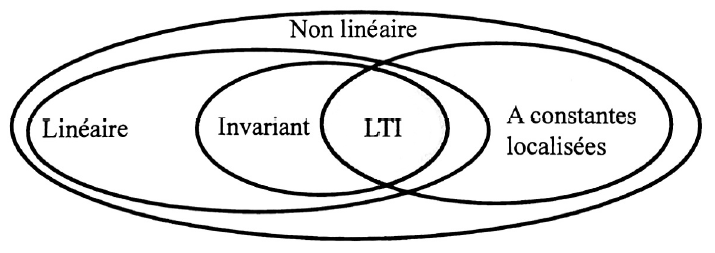
\includegraphics[scale=0.35]{1/graph1.png}
\end{center}

\section{Passage des EDP vers EDO }

Très souvent les systèmes étudiés sont régit par des équations aux dérivées partielles, pour faciliter leur étude on simplifie ces équations par approximation, car le modèle obtenu est de dimension infinie.
\[\vec{\omega}(x,y,z,t) \approx \sum_{i=1}^Nq_i(t)\vec{\eta}(x,y,z)\]

De plus La stabilité sera analysée sur l'aspect temporel car on ne peut pas avoir une dimension spatiale instable.

\begin{example}[Poutre flexible]
  On regarde les différent modes d'excitations, obtenus par la méthode des éléments finis.\\
Ceci permet donc de décrire le système dans la Base Modale.\\
\end{example}

\section{Forme générale de la représentation d'état}
Dans le cas général, les systèmes sont décrits par la représentation d'état :
\[\left\{ \begin{matrix}
      \dot{x} = f(x,t,u)\\
y = g(x,t,u)& \text{	avec, } & x\in \mathbb{R}^n\text{, }u\in \mathbb{R}^m\text{, }y\in \mathbb{R}^l
\end{matrix} \right.\]

\begin{exemple} Système LTV
\begin{align*}
  f(x,t,u) = A(t)x + B(t) u\\
  g(x,t,u) = C(t)x +D(t)u
\end{align*}
\end{exemple}

Ainsi la solution est noté $\chi (t,x_0)$, qui donne la valeur de $x$ à l'intsant t pour une condirtion initiale $x_0$


\begin{defin}
  La \emph{trajectoire} $\chi$ d'un système dynamique $\Sigma$ sur $\mathcal{D}\subset \R^n$ où $n$ est la dimension de $\Sigma$ , est une application :
  \[
    \chi: \R \times \mathcal{D} \to \mathcal{D}
  \]
  vérifiant les propriétés:
  \begin{enumerate}
  \item Continuité $\chi $ est continue sur $\R \times \mathcal{D}$ et $\forall x \in \mathcal{D}, \chi (\cdot,x) $ est dérivable sur $\R$
  \item Consistance $\chi(0,x) = x$
  \item Propriété de Groupe $ \chi(t,\chi(\tau,x))=\chi(t+\tau,x)$
  \end{enumerate}
\end{defin}

  \begin{rem}
    suivant la propriété 1. on a :
    \[
      \derivp[\chi(t,x)]{t} = f(\chi(t,x))
    \]
    et si on fixe $x=x_0$ à $t=0$ alors :
    \[
      \deriv[\chi(t,x_0)]{t}= f(\chi(t,x_0))
    \]
  \end{rem}
  \begin{defin}
    L'ensemble $\mathcal{D}$ dans lequel évolue la trajectoire est nommée \emph{espace de phase}

    Dans le cas causal, on se limite à
    $ \chi: \R_+ \times \mathcal{D} \to \mathcal{D}$.

    Pour $t$ fixé on note $\chi_t :=\chi(t,x) \mathcal{D}\to \mathcal{D}$
  \end{defin}
\begin{prop}
  L'application  $\chi_t$ ou $\chi_{-t}$ est un homéomorphisme:
  \begin{itemize}
  \item continu
  \item bijectif
  \item inverse continu
\end{itemize}

\end{prop}
\begin{proof}
  on montre l'injectivité et la surjectivité de $\chi$.
  La propriété 1. permet de montrer la continuité.
\end{proof}
\end{document}

%%% Local Variables:
%%% mode: latex
%%% TeX-master: "main"
%%% End:
